\documentclass[xcolor ={table,usenames,dvipsnames}]{beamer}
\usepackage[italian]{babel}
\usepackage{color}
\usepackage{txfonts}
\PassOptionsToPackage{dvipsnames}{xcolor}
\title{Duck Typing in Python}
\author{Author: Tommaso Puccetti}
\institute{Universit\`a  degli Studi di Firenze}
\date{21/12/2018}
%\usepackage{sansmathaccent}
\usetheme{Berlin} 
\useinnertheme{rounded}
\useoutertheme{miniframes} 
\setbeamercovered{dynamic}
\theoremstyle{definition}
\newtheorem{definizione}{Definizione}
\usepackage{tikz}
\usetikzlibrary{arrows}
\usepackage{subfigure}
\usepackage[procnames]{listings}
\usepackage{color}
\usepackage{jlcode}

\definecolor{keywords}{RGB}{255,0,90}
\definecolor{comments}{RGB}{0,0,113}
\definecolor{red}{RGB}{160,0,0}
\definecolor{green}{RGB}{0,150,0}

\lstset{language=Python, 
	backgroundcolor=\color{yellow},
	basicstyle=\fontsize{2}{4}\selectfont\ttfamily\scriptsize, 
	keywordstyle=\color{keywords},
	commentstyle=\color{comments},
	stringstyle=\color{green},
	showstringspaces=false,
	identifierstyle=\color{black},
	procnamekeys={def,class},
}

\begin{document}
	
	\begin{frame}
		\maketitle
			\begin{figure}[h!]
			\centering
			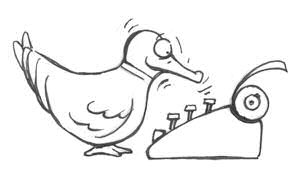
\includegraphics[scale=2]{img/cartoonduck.jpg}
			\label{Interfacce di un CS}
		\end{figure}
	\end{frame}

	\begin{frame}
		\frametitle{Index}
		\begin{enumerate}
			\item Introduction
			\item Python's semantic
			\item Type-checking
			\item Python Type checking
			 \begin{itemize}
					\item Dynamic typing
					\item Strong typing
					\item Annotations
				  \end{itemize}
			\item Object oriented
			\item Duck typing
				  \begin{itemize}
				  	\item Main idea
				  	\item Duck typing vs. Static typing
				  	\item Adding method to a class
				  \end{itemize}
			\item Conclusion
		\end{enumerate}
	\end{frame}

	\begin{frame}
		\frametitle{Introduction}
		Python is an \textit{\textbf{interpreted}}, \textit{\textbf{multi-paradigm}} language. It was initially designed by Guido van Rossum in 1991 and developed by Python Software Foundation. It supports:
		\begin{itemize}
			\item \textbf{Functional programming } (non pure);
			\item \textbf{Procedural programming};
			\item \textbf{Objected oriented}.
		\end{itemize}
		\begin{figure}[]
			\centering
			
\includegraphics[scale=0.3]{img/python.png}
			\label{Interfacce di un CS}
		\end{figure}
	\end{frame}

	\begin{frame}
		\frametitle{Python's semantic}
			Could be useful to first recall the difference between \textit{\textbf{strict}} and \textit{\textbf{lazy}} evaluation:
			\begin{enumerate}
				\item \textbf{Strict evaluation strategy}: the arguments of a function are fully evaluated to values before evaluating the function call (call by value);
				\item \textbf{Non-strict or Lazy evaluation:} arguments are evaluated only if it is needed in the function body (\textit{call by name})
			\end{enumerate}
			\textbf{Python}:		
			\begin{itemize}
				\item implements \textbf{strict evaluation};
				\item uses \textbf{whitespace indentation}, rather than curly brackets or keywords, to delimit blocks.
			\end{itemize}
	\end{frame}

	\begin{frame}[fragile]
		\frametitle{Strict evaluation: example}
		In Python we never get \textit{true} because  it force the evaluation of the function wich contains an infinite loop in the body:
		\begin{lstlisting}
			def infiniteLoop(x):
			    while True:
		           print("do something with x")
		        return x
				
			5 in [5, 10, infiniteLoop(5)]
		\end{lstlisting}
		If we write the same code in \textbf{haskell} we get the \textit{true} value:
		\begin{lstlisting}
			elem 5 [5, 10, noreturn 5]
		\end{lstlisting}
	\end{frame}

	\begin{frame}
		\frametitle{Type-checking }
			\textbf{Type checking} is the process of verifying and enforces the typing rules of a language.
		\begin{enumerate}
			\item \textbf{Dynamic vs. Static}
			\item \textbf{Weak vs. Strong}.
		\end{enumerate}
		\begin{figure}[h!]
			\centering
			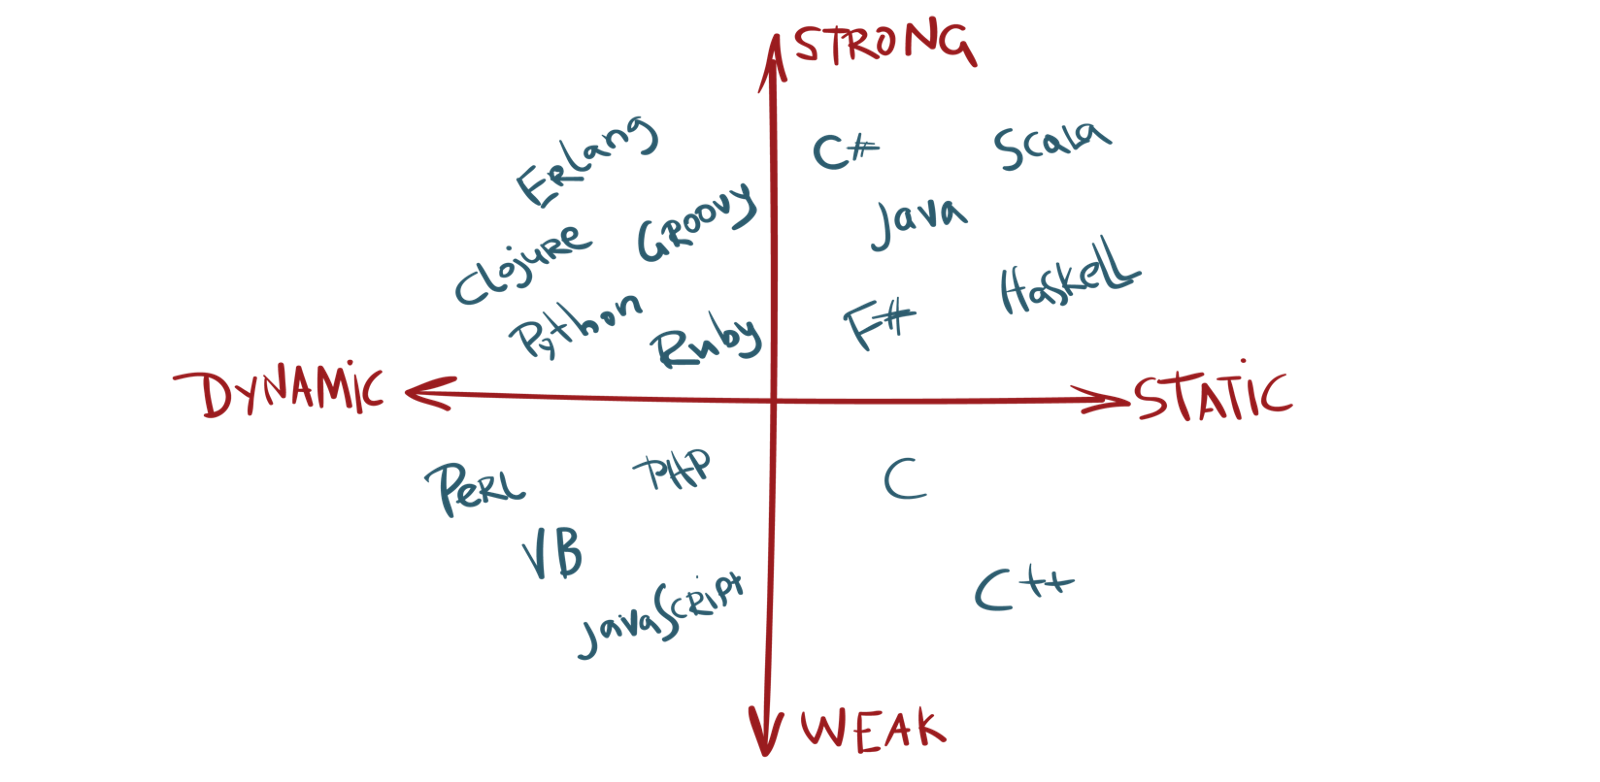
\includegraphics[scale=0.14]{img/classification.png}
		\end{figure}
	\end{frame}

	\begin{frame}
		\frametitle{Type-checking: static  }
		\textbf{Statically-typed languages}: type-checking is done at
		compile time, in order to guarantee the absence of run-time errors.
		\begin{itemize}
			\item \textbf{Advantages}:\begin{itemize}
				\item There is a formal proof of \textbf{type-safety};
				\item A large class of errors are caught earlier;
				\item Types guide code development;
				\item Types could be seen as documentation for the code.
			\end{itemize}
			\item \textbf{Disadvantages}: 
			\begin{itemize}
				\item Static typing is a constraint on the program structure;
				\item More code.
			\end{itemize}
		
		\end{itemize}
	\end{frame}

\begin{frame}
	\frametitle{Type-checking: dynamic}
	\textbf{Dynamically-typed languages:} dynamic
	type checking is the process of verifying type constraints at runtime,
	during execution.
	\begin{itemize}
		\item \textbf{Advantages}:
		\begin{itemize}
			\item These languages are more flexible;
			\item less code.
		\end{itemize}
		\item \textbf{Disadvantages}:
		\begin{itemize}
			\item Programs can fail at runtime due to type errors.
			\item It forces runtime checks to occur for every execution of the program, at any step of evaluation. The result is \textbf{less optimized} code.
		\end{itemize}
	\end{itemize}
 \end{frame}

\begin{frame}
	\frametitle{Type-checking: strong and weak}
	\begin{enumerate}
		\item \textbf{Strongly typed}: every expression is well typed;
			\begin{itemize}
				\item \textbf{Advantages}: 
			\end{itemize}
	\end{enumerate}
	
\end{frame}

	\begin{frame}
		\frametitle{Python type-checking}
			\begin{enumerate}
				\item Python type-checking is \textbf{dynamic}: 
				\begin{itemize}
					\item Variables have no type, only the object that a variable references has a type. \textbf{Variables are simply names pointing to objects};
					\item variables are not explicitly typed;
					\item objects have a type but it is determined at runtime;
				\end{itemize}
				\item Python is also \textbf{strongly typed}.
			\end{enumerate}
			
			Let's see the implications by some example.
	\end{frame}

	\begin{frame}[fragile]
		\frametitle{Python's dynamic typing example (1)}
			\begin{lstlisting} 
			if False:
				print(10+"ten") 
			else:
				print(10+10)
			\end{lstlisting}
			The first branch never execute, so the type checking ignore the type incongruency.
			
			If we try to execute \textbf{separately} the first branch, the type check raise a type error:
			
			\begin{lstlisting}[keywordstyle=\color{black},
			commentstyle=\color{black},
			stringstyle=\color{black}.]
			TypeError: unsupported operand type(s) for +: 'int' and 'str'
			\end{lstlisting}
	\end{frame}

	\begin{frame}[fragile]
		\frametitle{Python's dynamic typing example (2)}
		Another consequnce is that programmers are \textbf{free to bind the same names (variables) to different objects with a different type}. Then the following statements are perfectly legal:
		
		\begin{lstlisting}
		variable = 10
		variable = "ten"
		\end{lstlisting}
		
		So long as you only perform operations valid for the type the interpreter doesn't care what type they actually are. 
	\end{frame}

	\begin{frame}[fragile]
		\frametitle{Python's strong typing example}
		Python is not allowed to perform operations inappropriate to the type of the object: 
		\begin{lstlisting}
		print(10+"ten")
		\end{lstlisting}
		
		In a \textbf{weakly-typed} language, like PHP, the integer is forced to be a string and no type error is raised:
		\begin{lstlisting}
		$temp = "ten"; 
		$temp = $temp + 10; // no error caused
		echo $temp;
		\end{lstlisting}
	The output will be "ten10".
	\end{frame}

%\begin{frame}[fragile]
%		\frametitle{Some exceptions (1)}
%		There are some operations allowed even in case of type incongruence.\\
%		The\textbf{ boolean equivalence} is permitted in Python 2 and 3: 
%		
%		\begin{lstlisting}
%			print("10" == 10)
%			print("10" != 10)
%		\end{lstlisting}
%		Returning:
%		\begin{lstlisting}
%			False
%			True
%		\end{lstlisting}
%	\end{frame}

%	\begin{frame}[fragile]
%		\frametitle{Some exceptions (2)}
%		In Python 2 "\textit{grather than}" and \textit{"less than"} are permitted:
%		
%		\begin{lstlisting}
%		print("10">10)
%		print("10"<10)
%		\end{lstlisting}
%		
%		Returning:
		
%		\begin{lstlisting}
%		True
%		False
%		\end{lstlisting}
%		
%		Python 3 do not allowed to do "\textit{grather than}" and \textit{"less than"} controls like these.\\	
%	\end{frame}

	\begin{frame}[fragile]
		\frametitle{Annotations}
			Annotations were introduced in Python 3.0 and are the main way to add type hints to the code. We can annotate both \textbf{function} and \textbf{variable}.
			
			\begin{lstlisting}
				import math
				
				pi: float = 3.142
				
				def circumference(radius: float) -> float:
					return 2 * math.pi * radius
			\end{lstlisting}
			
			Type hints and annotations \textbf{\textit{do not add a real static typechecking}} in native Python so this should not effect the code performance.\\
	\end{frame}

	\begin{frame}
		\frametitle{Annotations: why use it?}
		\textbf{From PEP 484}:\\
		\textit{" <...>using type hints for performance optimizations is left as an exercise for the reader"}.\\
		
		\textbf{Advantages:}
		\begin{itemize}
			\item Type hints help document your code;
			\item Type hints improve IDEs and linters. This allows IDEs to offer better code completion and similar features.
		\end{itemize}
		\textbf{Disadvantages}
		\begin{itemize}
			\item Type hints take developer time and effort to add.
			\item Type hints introduce a slight penalty in start-up time.
		\end{itemize}
	\end{frame}

	\begin{frame}[fragile]
		\frametitle{Object oriented}
	\begin{lstlisting}
		class Duck():
			def __init__(self, name, colour):
				self.name = name
				self.colour = colour
			def quack(self):
				return "Quaaack"
			def fly(self):
				return "The duck is flying"
		
		donald = Duck("Donald","white")
				
		donald.name
		donald.colour
		donald.quack()
		donald.fly()
		\end{lstlisting}
	\end{frame}

	\begin{frame}[fragile]
		\frametitle{Object oriented: self}
		\begin{itemize}
			\item The first argument of every class method is always a reference to the current instance of the class (\textit{\textbf{self}}).
			\item The \textbf{\textit{self}} world is the equivalent of \textbf{\textit{this}} in \textbf{Java}. However Java do not requires to pass \textit{this} explicitly as a first parameter of a method: it could be used straight in the body.
			\item However self\textbf{ is not a reserved keyword} in Python, is just a strong convention.
		\end{itemize}
	%	\begin{lstlisting}[basicstyle=\fontsize{2}{4}\selectfont\ttfamily\tiny]
	%	class Duck():
	%		def __init__(myself, name, colour):
	%			myself.name = name
	%			myself.colour = colour
	%		def quack(myself):
	%			return "Quaaack"	
	%		def fly(myself):
	%			return "The duck is flying"
	%	\end{lstlisting}
	\end{frame}

	%\begin{frame}[fragile]
		%\frametitle{Object oriented (3)}
		%In Python \textbf{is not possible to define multiple constructor} for a class, still is possible
		%to define a default value if one is not passed.
	%	
	%	\begin{lstlisting}
	%	class Parrot():
	%		def __init__(self, name = "Perry"):
	%			self.name = name
	%	
	%	bird1 = Parrot()
	%	bird2 = Parrot("Jack")
	%	
	%	print(bird1.name)
	%	print(bird2.name)	\end{lstlisting}
	%	The output would be:\\
	%	"Perry"\\
	%	"Jack"
	%\end{frame}
	
	\begin{frame}[fragile]
		\frametitle{Object oriented: inheritance and polymorphism}
		\begin{lstlisting}[basicstyle=\fontsize{2}{4}\selectfont\ttfamily\tiny]
	class Person():
		def __init__(self, name, surname):
			self.name = name
			self.surname = surname
		def get_info(self):
			return self.name + " " + self. surname
	
	class Teacher(Person):
		def __init__(self, name, surname):
			Person.__init__(self, name, surname)
		def get_info(self):
			return self.name + " " + self. surname + " is a teacher"
	
	class Student(Person):
		def __init__(self, name, surname, id):
			Person.__init__(self, name, surname)
			self.id = id
		def get_info(self):
			return self.name + " " + self. surname + " is a student"
		def get_id(self):
			return self.id
		\end{lstlisting}
	\end{frame}
	
	

	\begin{frame}
		\frametitle{Duck typing}
		\textit{ If it looks like a duck, swims like a duck, and quacks like a duck, then it probably is a duck.}\\
		\begin{figure}[h!]
			\centering
			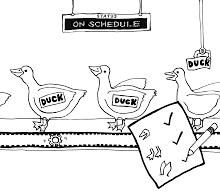
\includegraphics[scale=0.85]{img/duck.png}
			\label{Interfacce di un CS}
		\end{figure}
	\end{frame}

	\begin{frame}
		\frametitle{Duck typing: main idea}
		\textbf{Duck typing} is a concept related to dynamic typing in an object oriented language:
		\begin{itemize}
			\item Implementing duck typing you do not check types at all. Instead you check for the presence of a given method or attribute.
			\item \textbf{The idea is that it doesn't actually matter what type my data is - just whether or not i can do what i want with it.}
		\end{itemize}
	\end{frame}

	\begin{frame}[fragile]
		\frametitle{Duck typing: example (1)}
		%basicstyle=\fontsize{2}{4}\selectfont\ttfamily\tiny
		%class Bird():
		%def fly():
		%pass
		\begin{lstlisting}[]
		
		class Duck(Bird):
			def quack(self):
				return "Quaaack"
			def fly(self):
				return "The duck is flying"
		
		class Parrot(Bird):
			def quack(self):
				return "The parrot parrots a quack"
			def fly(self):
				return "The parrot is flying"
		
		class Man():
			def quack(self):
				return "The man parrots a quack too"

		\end{lstlisting}
	\end{frame}

	\begin{frame}[fragile]
		\frametitle{Duck typing: example (2)}
		\begin{lstlisting}	
		v = [Duck(), Parrot(), Man()]
		
		for i in v:
			print(i.quack())
		\end{lstlisting}
		Even if the istance of Man is not a subtype of the Bird class the type-checker do not raise any type error. The output would be:
		
		\begin{lstlisting}[keywordstyle=\color{black},
		commentstyle=\color{black},
		stringstyle=\color{black}.]	
		Quaaack
		The parrot parrots a quack
		The man parrots a quack too
		\end{lstlisting}
		
		
		
	\end{frame}

	\begin{frame}[fragile]
		\frametitle{Duck typing: example (3)}
		\begin{lstlisting}	
		for i in v:
			print(i.fly())
		\end{lstlisting}
		If we try to use the \textit{fly()} method  over the entire collection of objects an error is raised at runtime:
			\begin{lstlisting}[keywordstyle=\color{black},
		commentstyle=\color{black},
	stringstyle=\color{black}.]	
	The duck is flying
	The parrot is flying
	Traceback (most recent call last):
	File "/home/tommaso/git/ducktyping-tpl/code/ducklist.py", 
	line 23, in <module> print(i.fly())
	AttributeError: Man instance has no attribute 'fly'
		\end{lstlisting}
	\end{frame}

	\begin{frame}[fragile]
		\frametitle{Duck typing vs Static typing (1)}
		\begin{lstlisting}
		class Car:
			def __init__(self, engine):
				self.engine = engine
			def run():
				self.engine.turn_on()			
		\end{lstlisting}
		
		\begin{itemize}
			\item This is a classical example of \textbf{dependency injection};
			\item Note that my Car does not depends on any concrete implementation of engine: i'm just using a dependency injected instance of something that responds to a \textit{turn\_on} message;
			\item I could say my class Car depends on an interface. But I did not have to declare it. %\textbf{It is an "automatic interface".}\\
		\end{itemize}	
	\end{frame}
	
	\begin{frame}
		\frametitle{Duck typing vs Static typing (2)}
		In statically-typed language, like Java, if we want to pass different implementation of Engine, to the contructor of the Car class we had to:
		\begin{itemize}
			\item declare explicit interface (\textit{IEngine for example});
			\item declare its implementation (EngineV8 or ElectricEngine);
			\item explicitly define my Car parameter to be an implementation of IEngine.
		\end{itemize} 
		
	\end{frame}
	
	\begin{frame}[fragile]
		\frametitle{Duck typing vs Static typing (3)}	
		\begin{lstlisting}
		interface IEngine {
			void turnOn();
		}
		
		public class EngineV8 implements IEngine {
			public void turnOn() {
				// do something here
		}}
		
		public class Car {
			public Car(IEngine engine) {
				this.engine = engine;
				}
			public void run() {
				this.engine.turnOn();
				}
		}
		\end{lstlisting}
	\end{frame}

%	\begin{frame}[fragile]
%		\frametitle{Add method to a class}
	%		In Python there is a difference between:
	%	\begin{itemize}
	%		\item \textbf{Function};
	%		\item \textbf{Bound method}.
	%	\end{itemize}
		
		
	%	\begin{lstlisting}
	%	>>> def foo():
	%	...     print "foo"
	%	...
	%	>>> class A:
	%	...     def bar( self ):
	%	...         print "bar"
	%	...
	%	>>> a = A()
	%	>>> foo
	%	
	%	<function foo at 0x00A98D70>
	%	>>> a.bar
	%	<bound method A.bar of <__main__.A instance at 0x00A9BC88>>
	%	\end{lstlisting}
		
%	\end{frame}
	
	\begin{frame}[fragile]
		\frametitle{Add method to a class: example (1)}
		Due to the flexibility given by Duck typing is possible to poke a function into a class:
		\begin{lstlisting}	
			class Man():
				def __init__(self, name):
					self.name = name
				def quack(self):
					return "The man parrots a quack too"
			
			donald = Duck()
			charlie = Parrot()
			john = Man("John")
			jack = Man("Jack")
			
			v = [donald, charlie, john, jack]
					
			
		\end{lstlisting}
	\end{frame}
	
	\begin{frame}[fragile]
		\frametitle{Add method to a class: example (2)}
		\begin{lstlisting}
		def fly(self):
			return "Takes a plane"
		
		Man.fly = fly
		
		for i in v:
			print(i.fly())
		\end{lstlisting}
		Every istance of the Man class, even if previously instantiated, now has the fly method.
		\begin{lstlisting}[basicstyle=\fontsize{2}{4}\selectfont\ttfamily\tiny,keywordstyle=\color{black},
		commentstyle=\color{black},
		stringstyle=\color{black}.]	
			The duck is flying
			The parrot is flying
			John takes a plane
			Jack takes a plane
		\end{lstlisting}
	\end{frame}

	\begin{frame}[fragile]
		\frametitle{Add method to a single instance of a class (1)}
			It is possible to add a method to a single istance of a class but we have a problem: \textbf{the function is not automatically bound} when it's attached directly to an istance.
			
				\begin{lstlisting}
			john.fly = fly
			
			for i in v:
				print(i.fly())
				
   The duck is flying
   The parrot is flying
   Traceback (most recent call last):
   File "/home/tommaso/git/ducktyping-tpl/code/pokelist.py", line 33, 
   in <module> print(i.fly())
   TypeError: fly() takes exactly 1 argument (0 given)
			\end{lstlisting}
	\end{frame}
	
	\begin{frame}[fragile]
		\frametitle{Add method to a single instance of a class (2)}
			
		To properly bound the method  to "john" we had to use the module \textit{types}:
		
		\begin{lstlisting}
		import types
		
		john.fly = types.MethodType(fly, john)
		
		for i in v:
			print(i.fly())
		\end{lstlisting}
	\end{frame}

	\begin{frame}[fragile]
		\frametitle{Add method to a single instance of a class (3)}
			We still have an error but this time is caused by the istance "jack", proving that we added the method fly only to one istance of Man. 
		
		\begin{lstlisting}[keywordstyle=\color{black},
		commentstyle=\color{black},
		stringstyle=\color{black}.]
	The duck is flying
	The parrot is flying
	John takes a plane
	Jack takes a plane
	Traceback (most recent call last):
	File "/home/tommaso/git/ducktyping-tpl/code/pokelist.py",
	line 35, in <module>
	print(i.fly())
	AttributeError: Man instance has no attribute 'fly'
		\end{lstlisting}
	\end{frame}

\begin{frame}
	\frametitle{Conclusion}
\end{frame}

	

		
	
	

	
	
	
	
	
	
	
	
	
	
	
\end{document}